%-----------------------------------------------------------------------
% Beginning of chap2.tex
%-----------------------------------------------------------------------
%
%  AMS-LaTeX sample file for a chapter of a monograph, to be used with
%  an AMS monograph document class.  This is a data file input by
%  chapter.tex.
%
%  Use this file as a model for a chapter; DO NOT START BY removing its
%  contents and filling in your own text.
% 
%%%%%%%%%%%%%%%%%%%%%%%%%%%%%%%%%%%%%%%%%%%%%%%%%%%%%%%%%%%%%%%%%%%%%%%%


\chapter*{Lecture 10}
\addcontentsline{toc}{chapter}{Lecture 10}
\setcounter{chapter}{10}
\setcounter{section}{0}
\setcounter{equation}{0}
\setcounter{theorem}{0}
%\numberwithin{section}{chapter}
\numberwithin{equation}{chapter}
\numberwithin{theorem}{chapter}

%\epigraph{}{--- \textup{}}

So far we have seen aspects of the geometry of linear programming, discussed the feasible sets (polyhedra) and presented a useful duality theorem:
the optimal value of
\begin{equation}\label{eq:primal}\tag{P}
 \maximize \ip{\vct{c}}{\vct{x}} \ \subjto \mtx{A}\vct{x}\leq \vct{b}
\end{equation}
coincides with the optimal value of
\begin{equation}\label{eq:dual}\tag{D}
 \minimize \ip{\vct{b}}{\vct{y}} \ \subjto \mtx{A}^{\trans}\vct{y}=\vct{c}, \  \vct{y}\geq \zerovct,
\end{equation}
provided both~\eqref{eq:primal} and ~\eqref{eq:dual} have a finite solution. 

We now turn attention to algorithms for linear programming. We present the main idea behind the classical Simplex Algorithm and then discuss the more modern class of Interior Point Algorithms in more detail. The latter can be shown to be efficient in a very precise sense (polynomial time) and generalize to non-linear convex optimization.

\section{A first algorithm for linear programming}
For $\mtx{A}\in \R^{m\times n}$ and $\vct{b}\in \R^m$ let $P=\{\vct{x}\in \R^n\mid \mtx{A}\vct{x}\leq \vct{b}\}$ be the polyhedron of feasible points for~\eqref{eq:primal}. Recall that a vertex of $P$ is a zero-dimensional face of $P$, or equivalently, a point that cannot be written as convex combination of two distinct points of $P$.

If the optimization problem~\eqref{eq:primal} has a solution, then it can be shown (Problem Set 4) that there exists a vertex $\vct{x}^*$ such that
\begin{equation*}
 \max_{\vct{x}\in P} \ip{\vct{c}}{\vct{x}} = \ip{\vct{c}}{\vct{x}^*}.
\end{equation*}
Intuitively this is clear by looking at a picture, as in Figure~\ref{fig:vertex}: Move a hyperplane orthogonal to the objective $\vct{c}$ along this direction to the highest level that still intersects a polyhedron $P$, and try to imagine that this intersection {\em does not} contain a vertex. 

\begin{figure}[h!]
\centering
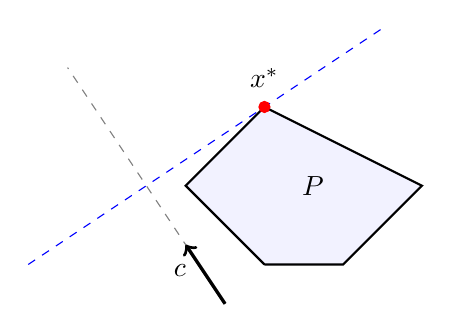
\begin{tikzpicture}[scale=1]
\draw[color=black, fill=blue!5, thick] (0,0)--(1,0)--(2,1)--(0,2)--(-1,1)--(0,0);
\draw[color=black!50,dashed] (-0.5,-0.5)--(-2.5,2.5);
\draw[color=black,very thick,->] (-0.5,-0.5)--(-1,0.25);
\draw[color=blue,dashed] (-3,0)--(1.5,3);
\filldraw[red] (0,2) circle (2pt);
\node (A1) at (-0.75,0.25)  [label=225:{$\vct{c}$}] {};
\node (A2) at (1,1)  [label=180:{$P$}] {};
\node (A3) at (0,2)  [label=90:{$\vct{x}^*$}] {};
\end{tikzpicture}
\caption{Geometry of linear programming} \label{fig:vertex}
\end{figure}

This crucial observation turns linear programming into a {\em finite} problem: we only have to test the objective function on the finite set of vertices to determine the maximizer. 
We have also seen (Problem Set 3) that the vertices can be identified as the solutions of the systems of equations
\begin{equation*}
 \mtx{A}_I\vct{x}=\vct{b}_I,
\end{equation*}
for which $\mtx{A}_I$ has full rank and $\vct{x}\in P$,
where $I\subset \{1,\dots,m\}$ is a subset of indices with $|I|=d$, and $\mtx{A}_I,\vct{b}_I$ are the matrix and vector arising from $\mtx{A}$ and $\vct{b}$ by taking the rows indexed by $I$. This gives a first primitive algorithm for solving the optimization problem~\eqref{eq:primal}. 

\begin{example}
 Consider the linear programming problem
 
 \begin{figure}[h!]
 \begin{minipage}{0.5\textwidth}
 \begin{align*}\label{eq:examples}
  \begin{split}
   \maximize &x_1-3x_2 \\
   \subjto &0.5x_1+x_2\leq 1\\
           &x_1+0.5x_2\leq 1\\
           &-x_1\leq 0\\
           &-x_2\leq 0\\
           &x_1\leq 1
  \end{split}
 \end{align*}
 \end{minipage}%
 \begin{minipage}{0.45\textwidth}
%  \begin{figure}[h!]
% \centering
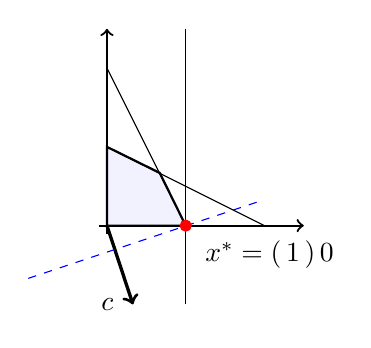
\begin{tikzpicture}[scale=1]
\draw[color=black, thick, ->] (0,-0.1)--(0,2.5);
\draw[color=black, thick, ->] (-0.1,0)--(2.5,0);
\draw[color=black, fill=blue!5, thick] (0,0)--(0,1)--(0.67,0.67)--(1,0)--(0,0);
\draw[color=black] (0,2)--(1,0);
\draw[color=black] (0,1)--(2,0);
\draw[color=black] (1,-1)--(1,2.5);
\draw[color=black,very thick,->] (0,0)--(0.33,-1);
\draw[color=blue,dashed] (-1,-0.67)--(2,0.33);
\filldraw[red] (1,0) circle (2pt);
\node (A1) at (1,0)  [label=-30:{$\vct{x}^*=\begin{pmatrix}1\\0\end{pmatrix}$}] {};
\node (A2) at (0.33,-1)  [label=180:{$c$}] {};
\end{tikzpicture}
%\end{figure}
\end{minipage}
\end{figure}
 
The matrix $\mtx{A}$ and vectors $\vct{b}$ and $\vct{c}$ are
\begin{equation*}
 \mtx{A} = \begin{pmatrix}
  0.5 & 1\\ 
  1 & 0.5\\
  -1 & 0\\
  0 & -1\\
  1 & 0
 \end{pmatrix},
\quad \vct{b} = \begin{pmatrix}
                 1\\ 1 \\ 0 \\ 0 \\ 1
                \end{pmatrix},
                \quad
                \vct{c} = \begin{pmatrix}
                           1 \\ -3
                          \end{pmatrix}.
\end{equation*}
We see that the minor $\mtx{A}_{\{3,5\}}=\begin{pmatrix} -1 & 0\\ 1 & 0\end{pmatrix}$, corresponding to the two parallel hyperplanes $x_1=0$ and $x_1=1$, is singular and does not define a vertex, while all other minors are invertible. For the minor $I=\{1,2\}$, $\mtx{A}_I\vct{x}=\vct{b}_I$ has the form
\begin{align*}
 0.5x_1+x_2 & = 1\\
 x_1+0.5x_2 & = 1,
\end{align*}
which has the solution $\vct{x}=(2/3,2/3)^{\trans}$. Since $\vct{x}$ also satisfies all the other inequalities, it is a vertex. In a similar fashion we can find all the vertices as the points
\begin{equation*}
 \vct{x}_1 = \begin{pmatrix} 2/3\\ 2/3\end{pmatrix}, \ \vct{x}_2 = \begin{pmatrix} 1\\ 0\end{pmatrix}, \ \vct{x}_3 = \begin{pmatrix} 0\\ 1\end{pmatrix}, \ \vct{x}_4 = \begin{pmatrix} 0\\ 0\end{pmatrix}.
\end{equation*}
The values of the objective function at these vertices are
\begin{equation*}
 \ip{\vct{c}}{\vct{x}_1} = -\frac{4}{3}, \ \ip{\vct{c}}{\vct{x}_2} = 1, \ \ip{\vct{c}}{\vct{x}_3} = -3, \ \ip{\vct{c}}{\vct{x}_4} = 0.
\end{equation*}
It follows that the optimization problem has the optimal value $1$ at $\vct{x}^*=(1,0)^{\trans}$.
\end{example}

Unfortunately, this method requires solving up to $\binom{m}{n}$ systems of linear equations, which can be exponential in $n$ in the worst case, making this method not practical. 

\begin{example}
Consider the hypercube
\begin{align*}
 -1&\leq x_1\leq 1\\
 &\cdots\\
 -1&\leq x_n\leq 1.
\end{align*}
It has $2^n$ vertices that need to be checked. Even though there are so many vertices, one can travel along edge between any two vertices in at most $n$ steps.
\end{example}


The simplex algorithm is a way to search through the vertices in a more clever way than just listing all of them. The idea is to start with a vertex and see if there is a vertex connected to it by an edge that has a bigger objective value. If not, we are done. If there is a neighbouring vertex, we move there and continue the process. We keep walking along the vertices of the feasible polytope until we find an optimal one.
\begin{figure}[h!]
\centering
 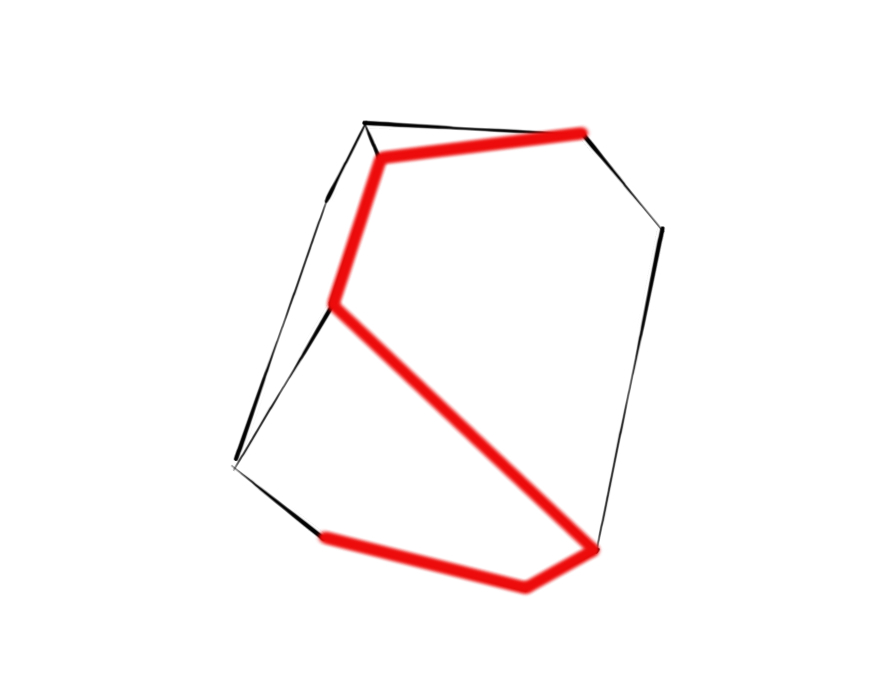
\includegraphics[width=0.35\textwidth]{images/durerpath.jpg}
 %\caption{A path along the edges of a polyhedron}
\end{figure}
The simplex algorithm is one of the most successful algorithms around and usually very fast, even though there examples that show that its worst case running time can be exponential.



% To implement this idea more rigorously, we transform the linear programming problem
% \begin{equation}\label{eq:opt}
%  \minimize \ip{\vct{c}}{\vct{x}} \quad \subjto \mtx{A}\vct{x}=\vct{b}, \ \vct{x}\geq 0.
% \end{equation}
% This can always be done. If we start with $\mtx{A}\vct{x}\leq \vct{b}$, then we can introduce {\em slack variables} $\vct{s}\geq 0$, so that the constraints become equivalent to
% \begin{equation*}
%  \mtx{A}\vct{x}+\vct{s}=\vct{b}, \quad \vct{s}\geq 0.
% \end{equation*}
%  We can now define
% \begin{equation*}
%  \vct{c}'=\begin{pmatrix} -\vct{c}\\ \vct{c}\\ \zerovct \end{pmatrix}, \ 
%  \mtx{A}'=\begin{pmatrix} \mtx{A} & -\mtx{A} & \mtx{I}\end{pmatrix}, \ \vct{x}'=\begin{pmatrix} \vct{x}^+ \\ \vct{x}^- \\ \vct{s}\end{pmatrix},
% \end{equation*}
% where $\vct{x}^+$ is the vector with entries $\max\{x_i,0\}$ and $\vct{x}^-$ the vector with entries $\max\{-x,0\}$. With this notation, we see that if $\vct{x}'$ is a solution of
% \begin{equation*}
%  \minimize \ip{\vct{c}'}{\vct{x}'} \quad \subjto \mtx{A}'\vct{x}'=\vct{b}, \ \vct{x}'\geq \zerovct,
% \end{equation*}
% then $\vct{x}=\vct{x}^+-\vct{x}^-$ is a solution of~\eqref{eq:opt}.

% %-----------------------------------------------------------------------
% % End of chap1.tex
% %-----------------------------------------------------------------------
